\documentclass[journal]{IEEEtran}
\usepackage[utf8]{inputenc}
\usepackage{graphicx}
\usepackage{amsmath}
\usepackage{siunitx}
\usepackage{xspace}
\usepackage{hyperref}
\usepackage{url}
\usepackage{cite}
\hyphenation{op-tical net-works semi-conduc-tor}

\begin{document}
	
	\title{Laboratorio 3: Lógica combinacional y Aritmética I}
	\author{Fiorella, Jonathan, Gerald}
	\date{Marzo 2021}
	
	\newcommand{\email}[1]{\href{mailto:#1}{#1}}
	
	\author{
		\IEEEauthorblockN
		{
			Fiorella Delgado León
			Jonathan Guzmán Araya,
			Gerald Valverde McKenzie
		}
		\IEEEauthorblockA{\\Instituto Tecnológico de Costa Rica}
		\IEEEauthorblockA{\\Área Académica Ingeniería en Computadores}
		
		\IEEEauthorblockA{\email{fio@gmail.com}}		
		\IEEEauthorblockA{\email{jonathana1196@gmail.com}}
		\IEEEauthorblockA{\email{gerald@gmail.com}}
	}
	
	% The paper headers
	\markboth{Laboratorio Taller de Diseño Digital, Semestre I~2021}%
	{Shell \MakeLowercase{\textit{et al.}}: Bare Demo of IEEEtran.cls for IEEE Journals}
	
	
	% make the title area
	\maketitle
	
	% As a general rule, do not put math, special symbols or citations
	% in the abstract or keywords.
	\begin{abstract}
		Este laboratorio sera.
	\end{abstract}
	% Note that keywords are not normally used for peerreview papers.
	\begin{IEEEkeywords}
		A, B, C
	\end{IEEEkeywords}
	
	\section{Introducción}
	
	Los circuitos combinacionales son aquellos en los que las salidas solo dependen solamente de las entradas, y no de ningún tipo de sincronización con señales de reloj, esto hace que los sistemas combinacionales sean generalmente rápidos. En sistemas digitales complejos, como los microprocesadores, los circuitos de lógica combinacional desempeñan un papel fundamental. La arquitectura de un microprocesador es como la que se observa en la Figura \ref{fig:microprocesador}.
	
	\begin{figure}[hbtp]
		\centering
		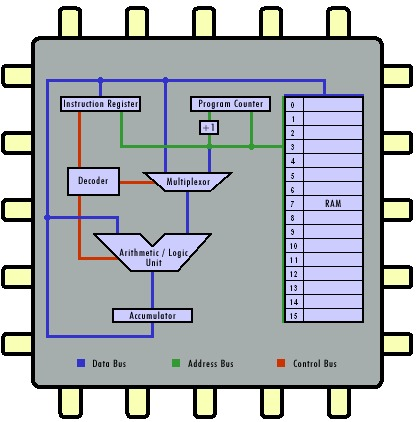
\includegraphics[scale = 0.5]{img/microprocesador.jpg}
		\caption{Arquitectura básica de un microprocesador \cite{Gonzalez2017}}
		\label{fig:microprocesador}
	\end{figure}

	Una función esencial de muchas computadoras (microprocesadores) y calculadoras es la realización de operaciones lógicas y aritméticas. Estas operaciones se efectúan en la unidad aritmética-lógica de una computadora, donde se combinan compuertas lógicas y flip-flops de manera que puedan sumar, restar, multiplicar y dividir números binarios \cite{Tocci2007}. Además de los operadores lógicos, la ALU cuenta con una serie de registros para almacenar los datos y bits de información sobre los resultados, también llamados banderas \cite{Garcia}. El símbolo de una ALU es como el de la Figura \ref{fig:simboloalu}.
	
	\begin{figure}[!htb]
		\centering
		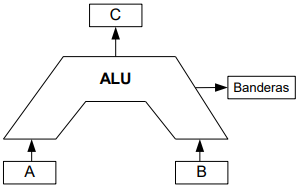
\includegraphics[scale = 0.5]{img/simboloalu.png}
		\caption{Símbolo ALU citar}
		\label{fig:simboloalu}
	\end{figure}
	
	La ALU es simplemente un operador, es decir solo realiza operaciones, esta no toma decisiones, acepta datos binarios que están almacenados en la memoria y ejecuta operaciones con estos datos, de acuerdo a las instrucciones que vienen de la unidad de control.
	
	Para realizar operaciones lógicas la ALU utiliza compuertas lógicas como:
	
	\begin{itemize}
		\item NOT: La Figura \ref{fig:NOT} muestra el símbolo para un circuito NOT, al cual se le conoce más comúnmente como INVERSOR, el INVERSOR afecta a una señal de entrada. Invierte (complementa) la señal de entrada en todos los puntos de la forma de onda, por lo que siempre que la entrada $= 0$, la salida $= 1$, y viceversa \cite{Tocci2007}.
		
		\begin{figure}[!htb]
			\centering
			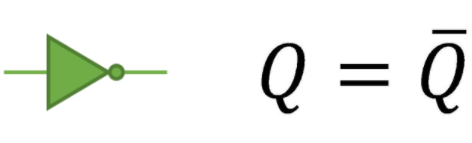
\includegraphics[scale = 0.35]{img/NOT.png}
			\caption{Compuerta NOT y su representación en álgebra de Boole \cite{logicbus}}
			\label{fig:NOT}
		\end{figure}
	
		\begin{table}[!htb]
			\centering
			\begin{tabular}{|c|c|}
				\hline
				Q & Q' \\
				\hline
				\hline
				0 & 1 \\
				\hline
				1 & 0 \\
				\hline
			\end{tabular}
			\caption{Tabla de verdad de la compuerta NOT}
			\label{tab:NOT}
		\end{table}
		
		\item AND: La Figura \ref{fig:AND} muestra el símbolo lógico para una compuerta AND de dos entradas. La salida de la compuerta AND es igual al producto AND de las entradas lógicas; es decir, $x=AB$. En otras palabras, la compuerta AND es un circuito que opera de manera que su salida esté en ALTO sólo cuando todas sus entradas se encuentren en ALTO. Para todos los demás casos, la salida de la compuerta AND estará en BAJO \cite{Tocci2007}.
		
		\begin{figure}[!htb]
			\centering
			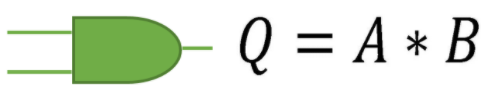
\includegraphics[scale = 0.3]{img/AND.png}
			\caption{Compuerta AND y su representación en álgebra de Boole \cite{logicbus}}
			\label{fig:AND}
		\end{figure}
	
		\begin{table}[!htb]
			\centering
			\begin{tabular}{|c|c|c|}
				\hline
				A & B & Q \\
				\hline
				\hline
				0 & 0 & 0 \\
				\hline
				0 & 1 & 0 \\
				\hline
				1 & 0 & 0 \\
				\hline
				1 & 1 & 1 \\
				\hline
			\end{tabular}
			\caption{Tabla de verdad de la compuerta AND}
			\label{tab:AND}
		\end{table}
		
		\item OR: La Figura \ref{fig:OR} muestra el símbolo lógico para una compuerta OR de dos entradas. Las entradas A y B son niveles lógicos de voltaje y la salida $x$ es un nivel lógico de voltaje cuyo valor es el resultado de la operación OR sobre A y B; es decir, $x = A + B$. En otras palabras, la compuerta OR opera de manera que su salida esté en ALTO, 1 lógico, si cualquiera de las entradas A o B o ambas se encuentran en el nivel 1 lógico. La salida de la compuerta OR estará en BAJO, 0 lógico, sólo si todas sus entradas están en 0 lógico \cite{Tocci2007}.
		
		\begin{figure}[!htb]
			\centering
			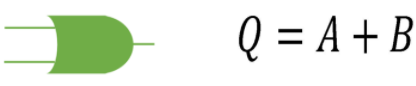
\includegraphics[scale = 0.35]{img/OR.png}
			\caption{Compuerta OR y su representación en álgebra de Boole \cite{logicbus}}
			\label{fig:OR}
		\end{figure}
	
		\begin{table}[!htb]
			\centering
			\begin{tabular}{|c|c|c|}
				\hline
				A & B & Q \\
				\hline
				\hline
				0 & 0 & 0 \\
				\hline
				0 & 1 & 1 \\
				\hline
				1 & 0 & 1 \\
				\hline
				1 & 1 & 1 \\
				\hline
			\end{tabular}
			\caption{Tabla de verdad de la compuerta OR}
			\label{tab:OR}
		\end{table}
		
		\item XOR: También llamada OR exclusiva, esta actúa como una suma binaria de un dígito cada uno y el resultado de la suma seria la salida. Otra manera de verlo es que con valores de entrada igual el estado de salida es 0 y con valores de entrada diferente, la salida será 1 \cite{logicbus}.
		
		\begin{figure}[!htb]
			\centering
			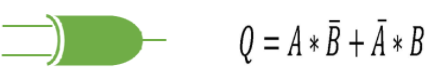
\includegraphics[scale = 0.4]{img/XOR.png}
			\caption{Compuerta XOR y su representación en álgebra de Boole \cite{logicbus}}
			\label{fig:XOR}
		\end{figure}
	
		\begin{table}[!htb]
			\centering
			\begin{tabular}{|c|c|c|}
				\hline
				A & B & Q \\
				\hline
				\hline
				0 & 0 & 0 \\
				\hline
				0 & 1 & 1 \\
				\hline
				1 & 0 & 1 \\
				\hline
				1 & 1 & 0 \\
				\hline
			\end{tabular}
			\caption{Tabla de verdad de la compuerta XOR}
			\label{tab:XOR}
		\end{table}
		
	\end{itemize}
	
	
	\section{Conclusiones}
	
	\section{Bibliografía}
	
	\bibliographystyle{IEEEtran}
	\bibliography{myref}
	
\end{document}